% fig07_cooling_b2.tex — cyclotron cooling time tau_c ∝ B^-2 across field strength.
% Compiled by the paper Makefile via `make figures` (pdflatex on the snippet).
%
% Data provenance (NO fabrication; commons @D g3) — Appendix D (app:cooling):
%   tau_c(B)/tau_c(1T) = (B/1T)^-2 (Larmor radiated power P ∝ B^2, inverted).
%     This is a normalized SCALING (dimensionless ratio), not an absolute
%     cooling time in seconds — the absolute prefactor (m^3 / q^4 etc.) is out
%     of scope (no equilibrium-T claim; app:cooling honest scope).
%   Registered verify-atom anchor (marker): tau_c(5T)/tau_c(1T) = 0.04
%     (cyclotron_cool_bratio(5,1)=0.04, PR #1015). 1/5^2 = 0.04 exactly.
%   The integer exponent -2 is the BLUE-MAX atom cyclotron_cool_bratio_exponent=2
%     (magnitude) / cyclotron_cool_bexponent=-2 (signed), PR #1094/#1015.
%   The dashed wrong-slope line (∝ B^-1) is the FALSIFIED negative control's
%     implied shape, shown to make the -2 vs -1 discrimination visible.
%
% Manual single-shot compile (debug):
%   pdflatex -interaction=nonstopmode -halt-on-error fig07_cooling_b2.tex
\documentclass[border=4pt]{standalone}
\usepackage{amsmath}
\usepackage{tikz}
\usepackage{pgfplots}
\pgfplotsset{compat=1.18}
\begin{document}
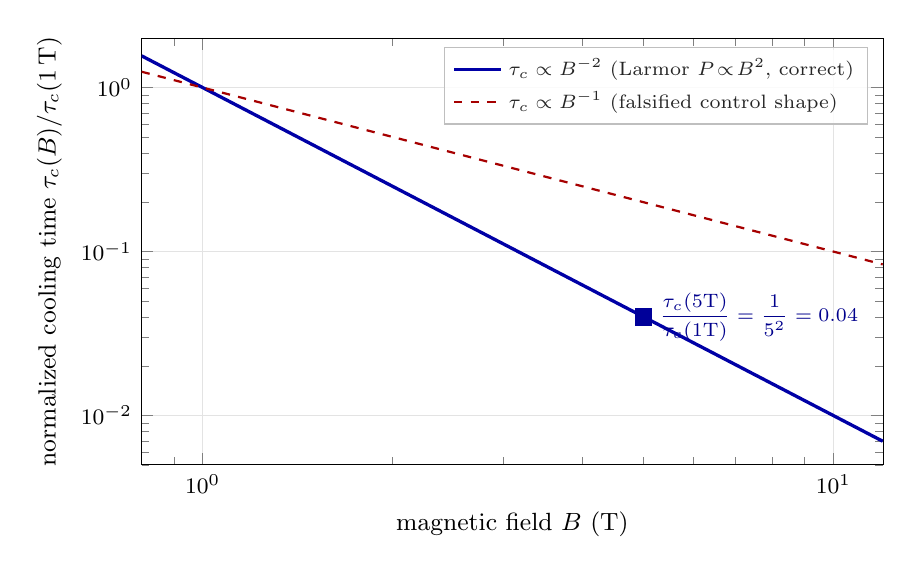
\begin{tikzpicture}
\begin{axis}[
  width=11cm, height=7cm,
  xmode=log, ymode=log,
  log basis x=10, log basis y=10,
  xlabel={magnetic field $B$ (T)},
  ylabel={normalized cooling time $\tau_c(B)/\tau_c(1\,\mathrm{T})$},
  xmin=0.8, xmax=12,
  ymin=5e-3, ymax=2,
  tick label style={font=\footnotesize},
  label style={font=\small},
  ymajorgrids, xmajorgrids, grid style={gray!22},
  legend style={font=\scriptsize, at={(0.98,0.98)}, anchor=north east,
    fill=white, fill opacity=0.85, draw=gray!50},
  legend cell align=left,
]
% --- correct B^-2 scaling ---
\addplot[blue!65!black, very thick, domain=0.8:12, samples=80] {x^(-2)};
\addlegendentry{$\tau_c\propto B^{-2}$ (Larmor $P\!\propto\!B^2$, correct)}
% --- wrong B^-1 (negative-control implied shape) ---
\addplot[red!65!black, dashed, thick, domain=0.8:12, samples=80] {x^(-1)};
\addlegendentry{$\tau_c\propto B^{-1}$ (falsified control shape)}
% --- registered anchor: tau_c(5T)/tau_c(1T) = 0.04 ---
\addplot[only marks, mark=square*, mark size=3pt, blue!60!black] coordinates {
  (5, 0.04)
};
\node[font=\scriptsize, anchor=west, text=blue!55!black]
  at (axis cs:5,0.04) {\;$\dfrac{\tau_c(5\mathrm{T})}{\tau_c(1\mathrm{T})}=\dfrac{1}{5^2}=0.04$};
\end{axis}
\end{tikzpicture}
\end{document}
